\documentclass[11pt,a4paper]{article}
\usepackage[utf8]{inputenc}
\usepackage[T1]{fontenc}
\usepackage[polish]{babel}
\usepackage{amsmath}
\usepackage{amsfonts}
\usepackage{amssymb}
\usepackage{graphicx}
\author{Paweł Cichowski}
\date{}
\title{SBD - projekt 2}

\begin{document}

\maketitle

\section*{Wprowadzenie}

Celem projektu było zaimplementowanie pliku o organizacji indeksowej, korzystając ze struktury B-drzewa. 

W programie zaimplementowane zostały operacje: dodawania rekordu, usuwania, aktualizacji. 

Operacje na pliku indeksowym są przeprowadzane z wykorzystaniem stron - każda strona zawiera indeksy opisujące dane oraz adresy stron potomnych. Strony są buforowane w pamięci w wektorze, który może zawierać do $h$ stron, czyli jedną gałąź drzewa.

Operacje na pliku danych zasymulowane są jako blokowe - odczyt lub zapis do dysku są wykonywane tylko przy sytuacji "cache miss". w pamięci buforowany jest jeden blok rekordów.

\section*{Opis działania programu}

\subsection*{Parametry pozycyjne}

Program obsługuje kilka parametrów pozycyjnych, pozwalających wybrać tryb pracy:

\begin{itemize}
\item -a, -{}-automatic <path> - program przyjmuje instrukcje z pliku testowego, opisanego w kolejnym punkcie
\item -i, -{}-interactive - program przyjmuje instrukcje z konsoli, w takim samym formacie co plik testowy
\item -v, -{}-verbose - program opisuje każdą wykonaną instrukcję
\end{itemize}

Program generuje również plik z logami w formacie csv. Zawiera on kolejne wykonane instrukcje i czas ich wykonania w milisekundach.

\newpage
\subsection*{Plik testowy}

Format pliku testowego:

\begin{verbatim}
rząd drzewa
maksymalny indeks losowo generowanych rekordów
instrukcja 1
instrukcja 2
...
\end{verbatim}

Dostępne instrukcje:

\begin{itemize}
\item i - insert rekordu o losowym kluczu
\item i <key> - insert rekordu o podanym kluczu
\item ip <key> - insert, po operacji wyprintowanie drzewa
\item d <key> - delete rekordu o podanym kluczu
\item dp <key> - delete, po operacji wyprintowanie drzewa
\item u <key> <identity> <name> <surname> <age> - update danych rekordu o podanym kluczu
\item p - printuje całe drzewo
\item end - koniec działania programu
\end{itemize}

\newpage
\section*{Wyniki eksperymentów}

Eksperyment polegał na dodaniu do pliku $n$ rekordów i zmierzeniu liczby operacji dyskowych, pamięciowych oraz czasu działania dla różnych wartości rzędu B-drzewa.

Danymi wejściowymi testów były: liczba rekordów: 10.000 oraz 1.000.000 dla rzędów drzewa: 2, 4, 16, 64, 256, 1024.

\subsubsection*{10.000 rekordów}

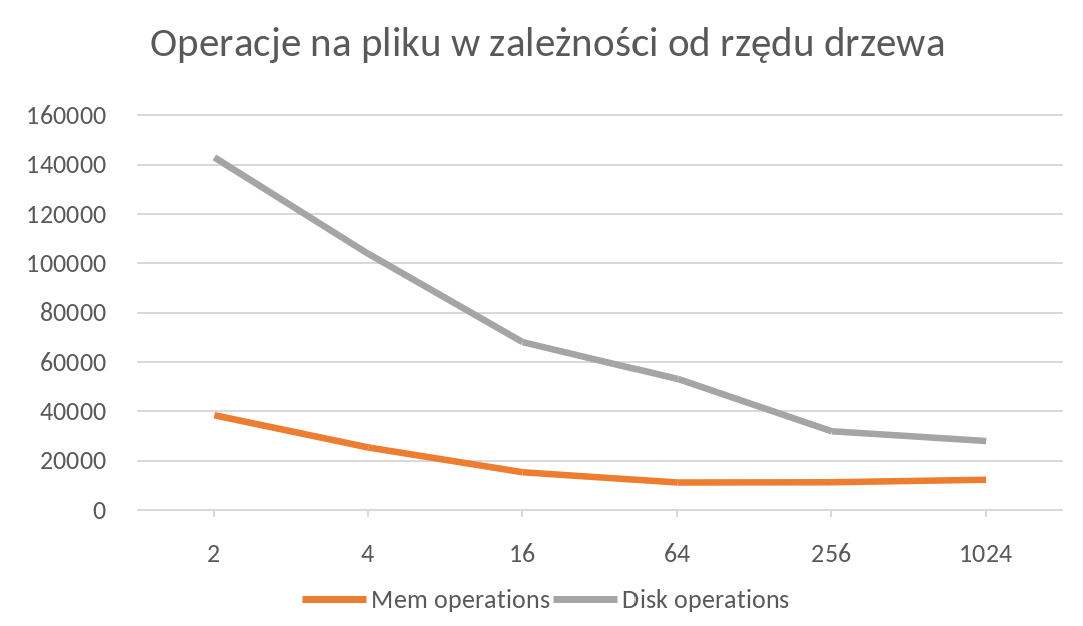
\includegraphics[scale=0.3]{sbd_operations_10k.png} 

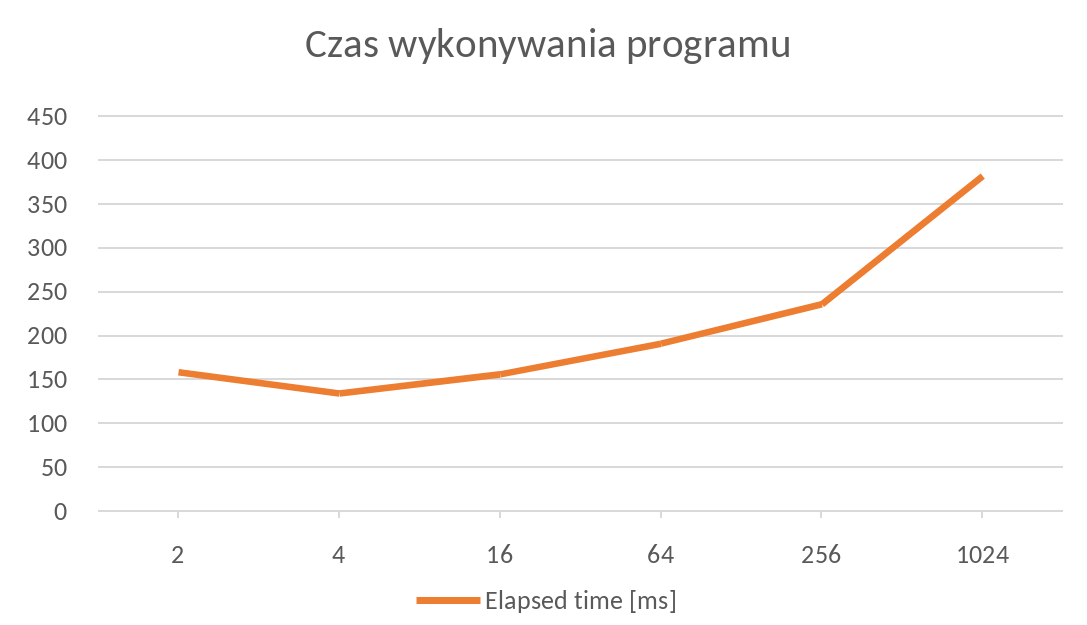
\includegraphics[scale=0.3]{sbd_time_10k.png} 


\subsubsection*{1.000.000 rekordów}

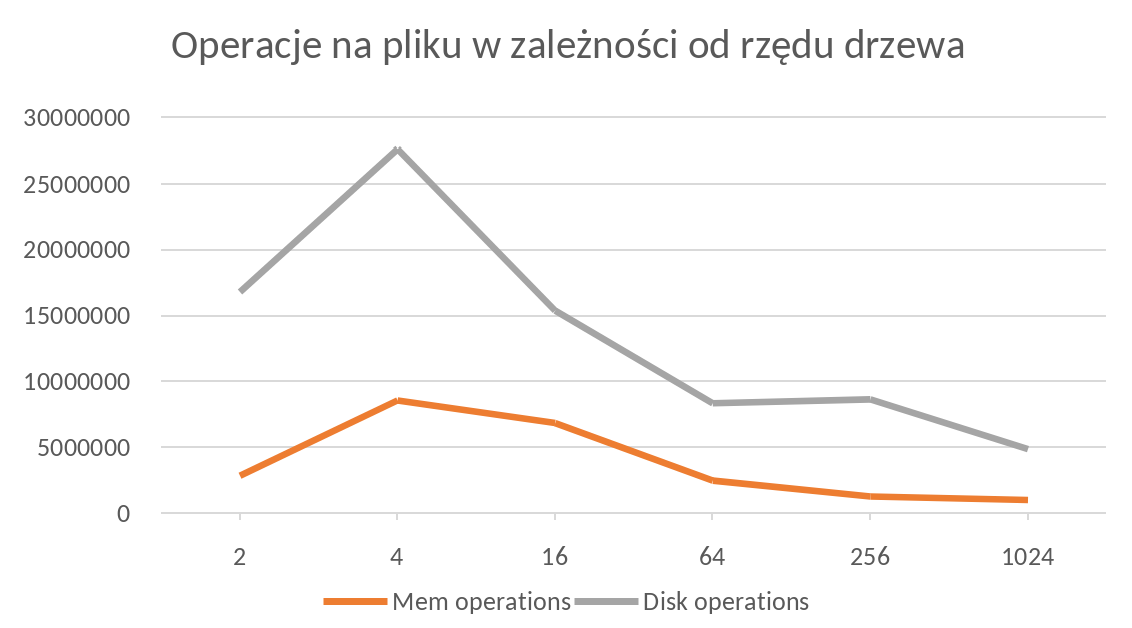
\includegraphics[scale=0.3]{sbd_operations_1m.png} 

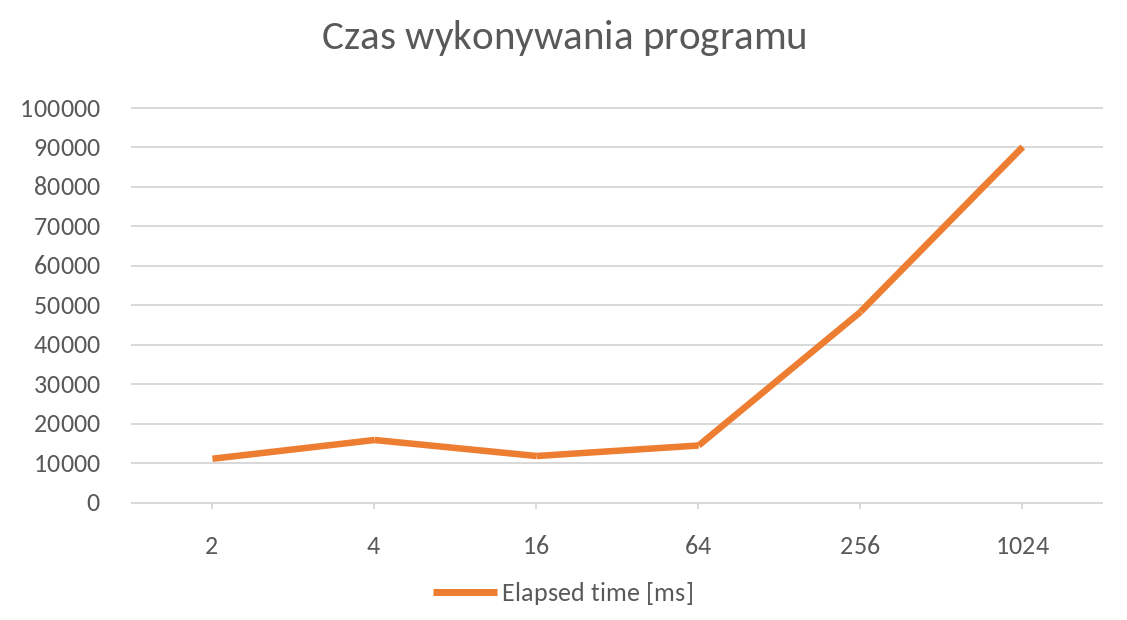
\includegraphics[scale=0.3]{sbd_time_1m.png} 

\section*{Wnioski}

Na podstawie przedstawionych wykresów postawione zostały poniższe wnioski:

\begin{itemize}
\item Większy rząd drzewa oznacza mniej zapisów do dysku, natomiast prowadzi do zwiększenia złożoności czasowej - większe strony są dłużej zapisywane.
\item Większy rząd oznacza również korzystniejszy stosunek między operacjami w pamięci a dyskowymi. Większe strony to częstszy "cache hit"
\newpage
\item Dla dużej liczby rekordów widoczna jest optymalna wartość rzędu drzewa - 64. Zachowuje kompromis między czasem działania a liczbą operacji dyskowych.
\end{itemize}

\end{document}